\section{Experimental Methodology}
\subsection{Implementation}
ICR observes the public tool catalog, concrete call arguments, returned
observations, and an append-only execution ledger. It never receives benchmark
injection labels, reference paths, task solutions, or judge verdicts. Tool
definitions supply input schemas, output annotations, categories, domains,
and declared substitutes. We retain PlanBench-XL's native retail
executor~\cite{planbenchxl}.

ICR separates a trusted backend compiler from the end-user agent. In the
PlanBench-XL deployment, the compiler may read the benchmark's released,
fixed retail relation to build a certificate index; neither ICR's language
model nor the native-agent control can inspect relation rows. Global,
observed-input, and type-only advice controls use the same compiler-side
catalog and index. Native-versus-ICR results therefore evaluate the deployed
recovery system, while matched advice controls isolate admission policy.

After an observed failure, the compiler enumerates alternative producers and
linked consumers, constructs their compatibility table, and computes the least
repair region. Admission requires lossless transport of supplied producer
arguments, a unique projection that binds the observed payload into the
consumer, and preservation of the original output schema. Generic
``data'' or ``object'' matches are rejected. At execution, a failed producer
interrupts the program before its consumer is dispatched; the original
failure and all recovery calls remain in the trace.

Candidate generation does not assume that a new failure is permanent. An
identical-call retry gate permits one further attempt unless persistence is
explicit; declared direct substitutions retain precedence when their concrete
inputs validate. Every matched online control uses the same catalog, retry
rule, retriever, executor, and failure trigger.

\subsection{Studies and Controls}
We evaluate structural optimality, boundary-value safety, and
online completion separately. Within each comparison, controls receive the
same frozen unit, public catalog, model, executor, and limits; reference paths
and judge labels enter only offline scoring.

\textbf{RQ1: structural exactness and joint choice.}
An exhaustive small-graph suite covers 40,824 fixed-assignment instances;
runtime audits enumerate all 16 regions of every recorded local assignment.
A local processor probe uses worst-propagation chains up to 50,000 nodes.
The multi-node study deduplicates 1,901 one-input TaskBench Multimedia and
Hugging Face graphs~\cite{taskbench}; each failed node receives 128 seeded
domain replacements, type equality defines compatibility, and external ports
remain immutable. Distinct graphs are cluster-bootstrapped and two additional
assignment seeds check stability.

For joint choice, every published operation receives two controlled format
variants from plain text, JSON, and protobuf, with fixed sampled costs and
unchanged operation identity. Exact DP, matched-information greedy, beam
controls, and the exhaustive oracle receive identical choices, boundaries,
costs, and compatibility tables. On 157 additional multi-input DAGs, variable
elimination and beams receive the same port-bound variants. Four-choice and
additional-seed runs test sensitivity. These interventions isolate interface
optimization; the executable catalog in RQ2 tests boundary-value effects.

\textbf{RQ2: boundary-value admission and native-agent recovery.}
PlanBench-XL supplies 327 retail queries, 185 typed tools, and a released
100-row read-only relation. Without reading task solutions, we enumerate
boundary-compatible paths of at most five calls. For the relational
certificate, all 136 unary edge dependencies are checked exhaustively on the
fixed relation; this is a finite-snapshot guarantee, not an inference about
future data. The compiler then indexes non-null row witnesses. Compilation
takes 0.172\,s and no tool or model calls. The index occupies 2.36\,MiB on disk
and 6.23\,MiB when parsed; 9,850 hash-and-lookup probes take a median
1.72\,$\mu$s each on one processor. Exhaustive native replay is used
only after compilation to audit all 31,565 path--input classifications. A
separate calibration/held-out replay rule provides an empirical comparator.

The online policies are native execution, type-only advice,
global-certificate advice, and ICR advice using the observed-input certificate.
A 29-prefix development study precedes an all-arm, reserved 21-task seed-42
holdout. The target population is explicit-blocker tasks with at least one
available globally certified local bypass, defined before model outcomes. Of 134 tasks untouched by
earlier development, 102 met this structural rule (76.1\%). Under seed 43 these
102 eligible tasks were frozen;
the first 30 served as diagnostics and the remaining 72 formed the sealed
independent-task confirmation. A separate 80-task schedule captures previously
unused input-only opportunities. Six prefixes form a pilot; the next 20 form
the sealed same-prefix comparison, with identical histories, states, and
failed actions. Its predeclared primary endpoint is restoration of the trusted
target value within 12 subsequent model turns; whole-task success is
secondary. An ancillary post-primary type-only arm replays the same 20
prefixes. Table~\ref{tab:study-map} separates their estimands and units.

\begin{table*}[t]
\centering\footnotesize\setlength{\tabcolsep}{5pt}
\caption{Evaluation cohorts and primary estimands.}
\label{tab:study-map}
\begin{tabular}{llll}
\toprule
\textbf{Study} & \textbf{Unit} & \textbf{Comparison} & \textbf{Primary endpoint}\\
\midrule
Structural oracle & 6,975 node failures in 1,901 graphs & DP, greedy, beams, oracle & Feasibility and minimum cost\\
Static certificate & 31,565 path--input pairs & Global, type only, observed input & Native-executor value equality\\
System confirmation & 72 globally certified-bypass tasks & Native vs. complete ICR advice & Whole-task completion\\
Admission holdout & 21 reserved tasks & Three certificate policies & Whole-task completion\\
Same-prefix confirmation & 20 input-only failure states & Three certificate policies & Target restoration within 12 turns\\
\bottomrule
\end{tabular}
\end{table*}

\subsection{Online Settings and Statistics}
All online arms use the same hosted endpoint, which reports the served-model
identifier \texttt{deepseek-flash}.
Temperature is zero, thinking is disabled, and the response cap is 4,096
tokens. PlanBench-XL retains its 100-step cap.
We use 100,000 paired template, task, or prefix bootstrap resamples (seed
20260924); reported 95\% intervals are percentile intervals. TaskBench graph
resamples are stratified by domain. Exact paired binary tests use the two-sided
McNemar test. The sealed 72-task and 20-prefix studies use task and matched
prefix as their respective units; pilots and ancillary controls are not pooled
with them. Every paired 72-task run reached a terminal benchmark outcome; no
task was omitted because of a missing model response.

\section{Results}
\subsection{Structural Recovery and Joint Choice}
The multi-node TaskBench study evaluates 892,800 fixed assignments on 1,901
distinct Multimedia and Hugging Face graphs. Among 28,933 feasible cases
whose replacement changes an adjacent interface, the least fixed point
matches an exhaustive subset oracle in every case. One and two rounds of
otherwise identical implication propagation miss 3,338 and 218 repairs,
respectively. The one-round recall gap is 11.5 percentage points (graph-bootstrap 95\%
interval [10.8, 12.3]); both extra assignment seeds give similar gaps.
A 50,000-node chain closes in 73.7\,ms median on one processor.

Each graph contributes one instance per possible failed node, giving 6,975
instances. All methods in Table~\ref{tab:joint-choice} receive identical candidates,
costs, immutable boundaries, and compatibility tables. ``Oracle match''
requires the same feasibility status and, when feasible, the same minimum cost.
\begin{table}[t]\centering\small\setlength{\tabcolsep}{4pt}
\caption{Joint repair on 1,901 TaskBench topologies.}
\label{tab:joint-choice}
\begin{tabular}{ccc}\toprule
\textbf{Method} & \textbf{Repairs found} & \textbf{Oracle match}\\\midrule
Forward greedy & 3,449/6,975 & 6,472/6,975\\
Beam width 2 & 3,745/6,975 & 6,786/6,975\\
Beam width 4 & 3,914/6,975 & 6,956/6,975\\
Beam width 8 & \textbf{3,933/6,975} & \textbf{6,975/6,975}\\
ICR joint tree DP & \textbf{3,933/6,975} & \textbf{6,975/6,975}\\
\bottomrule\end{tabular}\end{table}

Joint tree DP finds 484 feasible repairs missed by the matched-information
forward greedy rule, a gain of 6.9 percentage points (graph-bootstrap 95\% interval
[6.3, 7.6]); width-four beam misses 19. On 157 multi-input DAGs, exact
elimination matches the oracle at every one of 568 oracle-checkable positions.
With four implementations per operation, width-eight beams miss one to four
feasible DAG repairs across three independent seeds; elimination remains exact.
On three-choice chains, the exact DP scales from 0.040\,ms at three nodes to
117.4\,ms at 10,000 nodes, whereas exhaustive enumeration already takes
51.6\,ms at 11 nodes.
The graph experiments preserve each published operation's identity while
varying declared interface formats, isolating repair-scope optimization from
language-model generation.

\begin{figure*}[t]
\centering
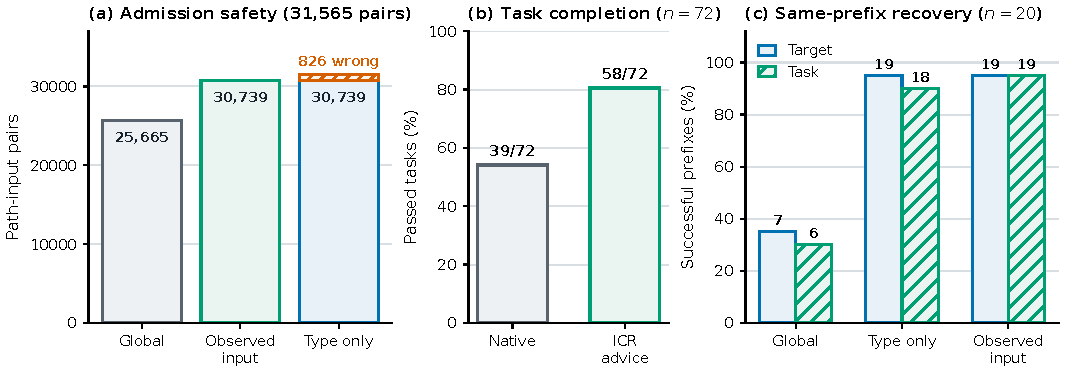
\includegraphics[width=.97\textwidth]{figures/results_overview.pdf}
\caption{PlanBench-XL results: (a) 31,565 path--input pairs; (b) 72 tasks; (c) 20 matched prefixes.}
\label{fig:results-overview}
\end{figure*}

\subsection{Observed-Input Certificate}
PlanBench-XL's independent retail executor yields 341 typed bypass paths
of two to five calls. Figure~\ref{fig:results-overview}(a) scores all 31,565
defined path--input pairs of the fixed read-only relation; here ``safe'' means
exact normalized output equality under the native executor on that snapshot.
The 9,250
failed-tool--input decisions below select at most one shortest route from
those pairs. The observed-input certificate recovers 5,074 safe
pairs inside the 59 paths rejected by global certification, without invoking
candidate paths at admission. Exhaustive native replay verifies every
classification. Among 9,250 failed-tool--input decisions, the shortest route
admitted by the observed-input certificate matches the native shortest-safe oracle in every case:
9,124 safe routes and 126 abstentions. Global certification finds 8,350
safe routes and abstains 900 times; type-only routing makes 126 wrong route
selections among these 9,250 decisions. The observed-input certificate thus recovers 774 safe decisions without
accepting the type-only errors.

\subsection{Native-Agent Recovery}
On 29 development first-failure prefixes, observed-input advice passes 26
continuations versus 20 for global advice (six paired gains, zero losses;
exact McNemar $p=0.031$). Four gains follow newly available packets. The
independent-task test below checks whole-trajectory transfer.

Table~\ref{tab:online-ablation} reports matched admission-rule controls: its
first row is whole-task pass and its second is trusted-target restoration
within 12 turns.
On the sealed 72-task seed-43 confirmation
(Fig.~\ref{fig:results-overview}(b)), ICR advice passes 58 tasks
versus 39 natively: 20 paired gains and one loss, a gain of 26.4 percentage
points (paired bootstrap 95\% interval [15.3, 37.5]; exact McNemar
$p=2.1\times10^{-5}$). Clustering by released reference path (49 groups)
and target datatype (19 groups) gives [16.1, 37.2] and [16.7, 35.5]
percentage-point intervals. Mean model requests differ by $-0.32$ per
task [$-3.99$, 3.32]. ICR emits 33 advice packets, and 17 of the 20 gains
contain a recovery event.
Across all 102 frozen eligible seed-43 tasks, including the 30-task diagnostic
stage, descriptive completion is 79/102 for ICR and 54/102 natively.

\begin{table}[t]
\centering\small\setlength{\tabcolsep}{4pt}
\caption{Matched PlanBench-XL online controls.}
\label{tab:online-ablation}
\begin{tabular}{ccccc}\toprule
\textbf{Frozen unit} & \textbf{Native} & \textbf{Global} & \textbf{Type only} & \textbf{ICR obs.}\\\midrule
21 tasks & 8/21 & \textbf{15/21} & \textbf{15/21} & \textbf{15/21}\\
20 prefixes & N/A & 7/20 & \textbf{19/20} & \textbf{19/20}\\
\bottomrule\end{tabular}
\end{table}

The prefix experiment starts from a native agent's already observed failed
state and isolates the three admission rules; it therefore has no separate
native continuation arm, shown as N/A in Table~\ref{tab:online-ablation}.

In the 21-task admission-rule holdout, global, type-only, and observed-input
advice emit 14, 15, and 15 packets, respectively. All 15 type-only packets in
this cohort pass the observed-input certificate, so the full-relation audit,
rather than this small task sample, exposes its 126 unsafe route decisions.
Of 62 frozen-order native captures, 26 met the
input-only failure rule; six formed the pilot and 20 the sealed same-prefix
confirmation (Fig.~\ref{fig:results-overview}(c)). Observed-input advice versus
global-certificate advice yields 12 paired local gains, no losses, a difference of 60 percentage
points (paired bootstrap 95\% interval [40, 80]; two-sided exact McNemar
$p=0.00049$). Whole-task success has 13 gains, no losses ($p=0.00024$).
Every local gain invokes a packet tool; four execute the full path. The
pilot enters neither test. In the ancillary type-only replay, all 20 first
paths coincide with and pass the observed-input certificate, yielding the
same local endpoint. Figure~\ref{fig:results-overview}(a) identifies the safety
distinction over the complete path--input relation.

